% !TEX encoding = UTF-8 Unicode

\documentclass[a4paper]{article}

\usepackage{color}
\usepackage{url}
\usepackage[T2A]{fontenc} % enable Cyrillic fonts
\usepackage[utf8]{inputenc} % make weird characters work
\usepackage{graphicx}

\usepackage[english,serbian]{babel}
%\usepackage[english,serbianc]{babel} %ukljuciti babel sa ovim opcijama, umesto gornjim, ukoliko se koristi cirilica

\usepackage[unicode]{hyperref}
\hypersetup{colorlinks,citecolor=green,filecolor=green,linkcolor=blue,urlcolor=blue}

%\newtheorem{primer}{Пример}[section] %ćirilični primer
\newtheorem{primer}{Primer}[section]

\begin{document}

\title{Analogni računari\\ \small{Seminarski rad u okviru kursa\\Tehničko i naučno pisanje\\ Matematički fakultet}}

\author{Aleksandar Končalović, Uroš Janković, Veljko Strugar, Veljko Josipović\\ kontakt email adresa autora}
\date{2.~novembar 2022.}
\maketitle

\abstract{
U ovom tekstu je ukratko prikazana osnovna forma seminarskog rada. Obratite pažnju da je pored ove .pdf datoteke, u prilogu i odgovarajuća .tex datoteka, kao i .bib datoteka korišćena za generisanje literature. Na prvoj strani seminarskog rada su naslov, apstrakt i sadržaj, i to sve mora da stane na prvu stranu! Kako bi Vaš seminarski zadovoljio standarde i očekivanja, koristite uputstva i materijale sa predavanja na temu pisanja seminarskih radova. Ovo je samo šablon koji se odnosi na fizički izgled seminarskog rada (šablon koji \emph{morate} da ispoštujete!) kao i par tehničkih pomoćnih uputstava. 

\tableofcontents

\newpage

\section{Uvod}
\label{sec:uvod}
Pre nastanka prvih digitalnih računara, za izračunavanja su se koristili \textbf{analogni računari}. Najstariji primer takvog računara je takozvani Mehanizam sa Antikitere za koji se veruje da datira iz drugog veka pre nove ere. \cite{antikitera}\\
Računari tog doba su se koristili za predviđanje raznih dešavanja u stvarnom svetu poput pomračenja Sunca i Meseca, tačnog vremena plime i oseke, a kasnije i u naučne i ratne svrhe.\\
Čak i nakon nastanka prvih digitalnih računara, analogni su jedno vreme bili smatrani moćnijim i bržim.

\section{Princip rada analognih računara}
Analogni računari vrše izračunavanja tako sto obrađuju kontinualne veličine. Iako se  za njihov rad najčešće koristi električna struja i napon, to nije nikakvo pravilo, i bilo koja kontinualna veličina može da se upotrebi. Te veličine su na primer: \begin{itemize}
				\item Količina vode u cevima
				\item Zategnutost opruga
				\item Intenzitet magnetne sile
				\item Vibracije tla kod seizmografa
				\item Visina vode kod mašine za predvidjanje plime i oseke \cite{tide}
				\item Položaj zubčanika
				\item Položaj čekrka
				\item Temperatura raznih supstanci
			\end{itemize}
			
\bigskip

    \begin{primer}
    Uzmimo kao primer operaciju sabiranja dva borja koristeći količinu vode u posudama.\\
    Da bismo sabrali dva broja, recimo 3 i 5, poterebno je da imamo tri identične čaše sa skalom za merenje nivoa vode u čaši. Sabiranje možemo izvrsiti prateći sledeći postupak:\begin{enumerate}
        \item U prvu čašu nalijemo vode do trećeg podeoka (za broj 3).
        \item U drugu čašu nalijemo vodu do petog podeoka (za broj 5).
        \item Prelijemo sadržaj obe čaše u treću času koju smo ostavili praznu.
        \item Očitamo visinu vode tako što gledamo do kog podeoka je stigla.
        \item Uočavanjem da je visina vode stigla do osmog podeoka (za broj 8) dobili smo rezultat sabiranja.
    \end{enumerate}
    \end{primer}
    
\bigskip

    \begin{primer}
    Za množenje dva broja možemo koristiti električnu struju, napon i otpor.\\
    Da bismo pomnožili dva broja, recimo 3 i 5, poterebno je da imamo voltmetar i električno kolo koje se sastoji od strujnog generatora i promenljivog otpornika. Množenje možemo izvrsiti prateći sledeći postupak:\begin{enumerate}
        \item Podesimo strujni generator tako da generiše električnu struju od tri ampera (za broj 3).
        \item Podesimo promenljivi otpornik tako da mu otpor bude pet oma (za broj 5).
        \item Postavimo pipalice voltmetra na krajeve otpornika.
        \item Očitamo napon na voltmetru.
        \item Uočavanjem da je napon očitan na volmetru jednak petnaest volti (za broj 15) dobili smo rezultat množenja.
    \end{enumerate}
    \centering Ovaj postupak koristi formulu
    \centering $$ U = R*I $$\\
    \centering za računanje proizvoda.
    \end{primer}


\section{Hidrointegrator Mike Alasa}	
\label{sec:hidrointegrator}

Hidrointegrator Mihaila Petrovića Alasa je prva analogna računska mašina koja radi na principu kretanja tečnosti. Petrovićev rad na ovom uređaju najavio je još 1896. profesor mehanike na Velikoj školi u Beogradu Ljubomir Klerić.\\
Usavršena verzija, koja se smatra završnim rešenjem hidrointegratora, opisana je u američkom časopisu za matematiku (eng.~{\em American Journal of Mathematics}) 1899. godine.\cite{hidrointegrator}\\
Na slici \ref{fig:h1} prikazana je skica hidrointegratora. 

\bigskip

\begin{figure}[h!]
\begin{center}
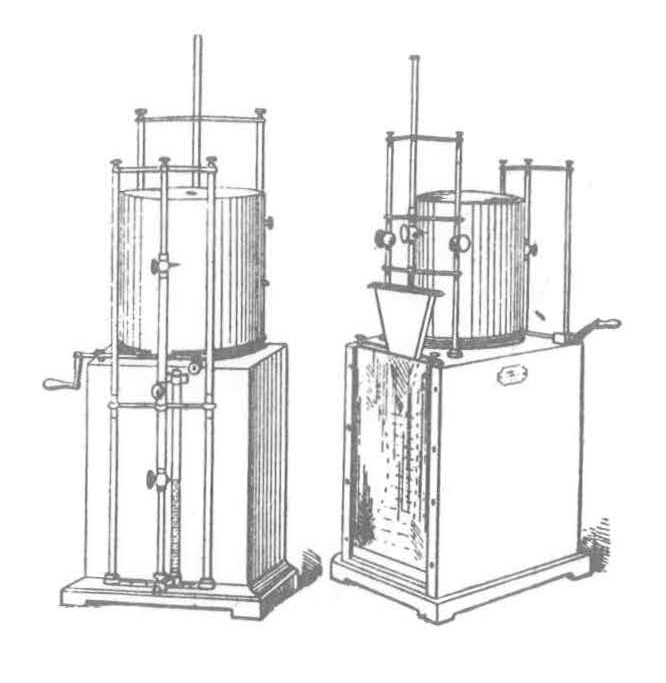
\includegraphics[scale=1.5]{h1.jpg}
\end{center}
\caption{Petrovićeva skica hidrointegratora. }
\label{fig:h1}
\end{figure}

\bigskip





\section{Slike i tabele}
\label{slike_i_tabele}

Slike i tabele treba da budu u svom okruženju, sa odgovarajućim naslovima, obeležene labelom da koje omogućava referenciranje. 

\begin{primer} Ovako se ubacuje slika. Obratiti pažnju da je dodato i 
\begin{verbatim}
\usepackage{graphicx}
\end{verbatim}

\begin{figure}[h!]
\begin{center}
\includegraphics[scale=0.75]{pande.jpg}
\end{center}
\caption{Pande}
\label{fig:pande}
\end{figure}

Na svaku sliku neophodno je referisati se negde u tekstu. Na primer, na slici \ref{fig:pande} prikazane su pande. 
\end{primer}

\begin{primer} I tabele treba da budu u svom okruženju, i na njih je neophodno referisati se u tekstu. Na primer, u tabeli \ref{tab:tabela1} su prikazana različita poravnanja u tabelama.

\begin{table}[h!]
\begin{center}
\caption{Razlčita poravnanja u okviru iste tabele ne treba koristiti jer su nepregledna.}
\begin{tabular}{|c|l|r|} \hline
centralno poravnanje& levo poravnanje& desno poravnanje\\ \hline
a &b&c\\ \hline
d &e&f\\ \hline
\end{tabular}
\label{tab:tabela1}
\end{center}
\end{table}

\end{primer}





\section{Prvi naslov}
\label{sec:naslov1}


Ovde pišem tekst. 
Ovde pišem tekst. 
Ovde pišem tekst. 
Ovde pišem tekst. 
Ovde pišem tekst. 
Ovde pišem tekst. 
Ovde pišem tekst. 
Ovde pišem tekst. 


\subsection{Prvi podnaslov}
\label{subsec:podnaslov1}

Ovde pišem tekst. 
Ovde pišem tekst. 
Ovde pišem tekst. 
Ovde pišem tekst. 
Ovde pišem tekst. 
Ovde pišem tekst. 
Ovde pišem tekst. 

\subsection{Drugi podnaslov}
\label{subsec:podnaslov2}

Ovde pišem tekst. 
Ovde pišem tekst. 
Ovde pišem tekst. 
Ovde pišem tekst. 
Ovde pišem tekst. 
Ovde pišem tekst. 

\section{Drugi naslov}
\label{sec:naslov2}

Ovde pišem tekst. 
Ovde pišem tekst. 
Ovde pišem tekst. 
Ovde pišem tekst. 

\subsection{... podnaslov}
\label{subsec:podnaslovN}

Ovde pišem tekst. 
Ovde pišem tekst. 
Ovde pišem tekst. 
Ovde pišem tekst. 
Ovde pišem tekst. 
Ovde pišem tekst. 

\section{n-ti naslov}
\label{sec:naslovN}

Ovde pišem tekst. 
Ovde pišem tekst. 
Ovde pišem tekst. 
Ovde pišem tekst. 
Ovde pišem tekst. 

\subsection{... podnaslov}
\label{subsec:podnaslovK}

Ovde pišem tekst. 
Ovde pišem tekst. 
Ovde pišem tekst. 
Ovde pišem tekst. 
Ovde pišem tekst. 

\subsection{... podnaslov}
\label{subsec:podnaslovM}

Ovde pišem tekst. 
Ovde pišem tekst. 
Ovde pišem tekst. 
Ovde pišem tekst. 
Ovde pišem tekst. 

\section{Elektronski analogni r\v{c}unari}
		\label{sec:naslovM}

			\par Mehani\v{c}ki analogni ra\v{c}unari su imali mnoge mane:
			\begin{itemize}
				\item bili su glomazni i te\v{s}ki za odr\v{z}avanje
				\item brzina izra\v{c}unavanja bila je strogo ograni\v{c}ena momentom inercije komponenata
				\item preciznost je bila limitirana na svega nekoliko procenata usled mrtvog hoda
				\item vreme potrebno za pode\v{s}avanje ra\v{c}unara za specifi\v{c}ne probleme bilo je veoma veliko jer je potrebno izvr\v{s}iti veliki broj prespajanja
			\end{itemize}
			\par Ove osobine su bile razlog za kratak \v{z}ivotni vek mehani\v{c}kih analognih ra\v{c}unara i ra\dj{}anja ideje o elektronskim analognim ra\v{c}unarima koji su brzo postali veoma uticajani.
			\par Prvi elektronski analogni r\v{c}unar implementirao je nema\v{c}ki nau\v{c}nik Helmut Holzer tokom Drugog svetskog rata tokom svog rada na kontroli letenja namenskih dalekometnih artiljerijskih oru\v{z}ja za strategijsko bombardovanje \v{s}to je zahtevalo ogroman broj izra\v{c}unavanja. \cite{Holzer}
			\par Klju\v{c}ni deo ovakvih ra\v{c}unara je \emph{operacioni poja\v{c}ava\v{c}}: stabilan linearni ure\dj{}aj prvobitno dizajniran za potrebe ameri\v{c}ke transkontinentalne telefonije. Druga bitna komponenta ovih ra\v{c}unara bio je potenciometar koeficijenta kori\v{s}\'{c}en da obezbeti odgovaraju\'{c}e skaliranje elektronskih analognih promenljivih.
			\par Razlozi zbog kojih je popularnost ranih elektronskih analognih ra\v{c}unara brzo poarsla su:
			\begin{itemize}
				\item manja veličina u odnosu na mehani\v{c}ke analogne ra\v{c}unare
				\item lak\v{s}a prenosivost
				\item ni\v{z}a cena
				\item  ve\'{c}a brzina
			\end{itemize}
			Jo\v{s} jedan od razloga njihove popularnosti je taj \v{s}to su ubrzo postali nerazdvojni deo istra\v{z}ivanja i razvoja u vojsci, vazduhoplovstvu i sektorima za in\v{z}enjerska istra\v{z}ivanja, \v{s}to pokazuje i tabela \ref{tab:tableEAR} \cite{table}
		
			\begin{table}[h!]
				\begin{center}
					\begin{tabular}{| p{2cm} | p{4cm} | p{1cm} | p{4cm} |}
						\hline
						Projekat / ma\v{s}ina & Razvojni centar & Datum & Namena \\
						\hline
						Projekat \emph Ciklon & Ameri\v{c}ka mornarica & 1946 & analogno - digitalno pra\'{c}enje performansi \\
						\hline
						Projekat \emph Tajfun & Ameri\v{c}ka mornarica / Ameri\v{c}ka radijska korporacija & 1947 & Jednostruka namenska ma\v{s}ina \\
						\hline
						MIT simulator letenja & Ameri\v{c}ka mornarica/MIT & 1948- 1958 & \\
						\hline
						RAND analogni ra\v{c}unar & RAND korporacija & 1948 & Pravljenje Rand analognog ra\v{c}unaram \\
						\hline
						GEDA/BEAC &  Ameri\v{c}ka avijacija & 1950- 1955 & Simulacija lansiranja projektila \\
						\hline
						LACE & Engleska elektroindustrija & 1953- 1956 & Op\v{s}ta namena/simulacija lansiranja projektila \\
						\hline
					\end{tabular}
					\label{tab:tableEAR}
				\end{center}
			\end{table}

\section{Zaključak}
\label{sec:zakljucak}

Ovde pišem zaključak. 
Ovde pišem zaključak. 
Ovde pišem zaključak. 
Ovde pišem zaključak. 
Ovde pišem zaključak. 
Ovde pišem zaključak. 
Ovde pišem zaključak. 
Ovde pišem zaključak. 
Ovde pišem zaključak. 
Ovde pišem zaključak. 
Ovde pišem zaključak. 
Ovde pišem zaključak. 


\addcontentsline{toc}{section}{Literatura}
\appendix

\iffalse
\bibliography{seminarski} 
\bibliographystyle{plain}
\fi

\begin{thebibliography}{9}

\bibitem{laski2009software} J. Laski and W. Stanley. \emph{Software Verification and Analysis}. Springer- Verlag, London, 2009.

\bibitem{gcc} Free Software Foundation. GNU gcc, 2013. on-line at: http://gcc. gnu.org/.

\bibitem{antikitera} Jo Marchant, "Archimedes and the 2000-year-old computer" New Scientist, 12 December 2008.

\bibitem{tide} E G Fischer (1912), "The Coast and Geodetic Survey Tide Predicting Machine No. 2".

\bibitem{hidrointegrator} Srpska akademija nauka i umetnosti, "Hidrointegrator Mihaila Petrovića Alasa". Pristupljeno 6.11.2022.

\bibitem{Holzer} Thomas H. Lange "Peenemuende, Analyse einer Technologieentwicklung im Dritten Reich", VDI-Verlag, 2006.
			
\bibitem{table} Bissell, C.C. (2004). A great disappearing act: the electronic analogue computer. In: IEEE Conference on the History of Electronics, 28-30 Jun 2004, Bletchley, UK.


\end{thebibliography}


\appendix
\section{Dodatak}
Ovde pišem dodatne stvari, ukoliko za time ima potrebe.
Ovde pišem dodatne stvari, ukoliko za time ima potrebe.
Ovde pišem dodatne stvari, ukoliko za time ima potrebe.
Ovde pišem dodatne stvari, ukoliko za time ima potrebe.
Ovde pišem dodatne stvari, ukoliko za time ima potrebe.


\end{document}
